\documentclass[a4paper]{article}
% \usepackage{thesis}
% define the title
\author{Glen Berseth\\
\textbf{Reviewed by:} Afshin Haidari-Khabbaz}
\title{Generalized Biped in Bullet}

\usepackage{epsfig}
\usepackage{amssymb}
\usepackage{amsmath}
\usepackage{amsfonts}
\usepackage{xspace}
\usepackage{named}
\usepackage{hyperref}
\usepackage{booktabs}
\usepackage{float}
\usepackage{wrapfig}
% \usepackage{cite}
%\usepackage{jneurosci}
% \usepackage{natbib}

\usepackage{graphicx}

\usepackage{algorithm2e}
% \usepackage{algorithm}
\usepackage{multirow}
\usepackage{verbatim}
\usepackage{soul}
\usepackage{array}
\setlength\extrarowheight{2pt} % or whatever amount is appropriate

% I am having a hell of a time getting text colouring working in this document
\usepackage[table]{xcolor}
\usepackage{array,hhline}
\usepackage{tikz}
\usetikzlibrary{calc}
\usetikzlibrary{decorations.pathmorphing}
% \usepackage{beamer}
\usepackage{caption}
\usepackage{siunitx}
% \sisetup{output-exponent-marker = E,round-mode = figures, round-precision = 3,
%  scientific-notation = true}
\sisetup{fixdp,dp=3}

% \usepackage[framed,numbered,autolinebreaks,useliterate]{mcode}

% \documentclass{minimal}
\usepackage{soul}
\usepackage{tikz}
\usetikzlibrary{calc}
\usetikzlibrary{decorations.pathmorphing}

\makeatletter

\newcommand{\defhighlighter}[3][]{%
  \tikzset{every highlighter/.style={color=#2, fill opacity=#3, #1}}%
}

\defhighlighter{yellow}{.5}

\newcommand{\highlight@DoHighlight}{
  \fill [ decoration = {random steps, amplitude=1pt, segment length=15pt}
        , outer sep = -15pt, inner sep = 0pt, decorate
        , every highlighter, this highlighter ]
        ($(begin highlight)+(0,8pt)$) rectangle ($(end highlight)+(0,-3pt)$) ;
}

\newcommand{\highlight@BeginHighlight}{
  \coordinate (begin highlight) at (0,0) ;
}

\newcommand{\highlight@EndHighlight}{
  \coordinate (end highlight) at (0,0) ;
}

\newdimen\highlight@previous
\newdimen\highlight@current

\DeclareRobustCommand*\highlight[1][]{%
  \tikzset{this highlighter/.style={#1}}%
  \SOUL@setup
  %
  \def\SOUL@preamble{%
    \begin{tikzpicture}[overlay, remember picture]
      \highlight@BeginHighlight
      \highlight@EndHighlight
    \end{tikzpicture}%
  }%
  %
  \def\SOUL@postamble{%
    \begin{tikzpicture}[overlay, remember picture]
      \highlight@EndHighlight
      \highlight@DoHighlight
    \end{tikzpicture}%
  }%
  %
  \def\SOUL@everyhyphen{%
    \discretionary{%
      \SOUL@setkern\SOUL@hyphkern
      \SOUL@sethyphenchar
      \tikz[overlay, remember picture] \highlight@EndHighlight ;%
    }{%
    }{%
      \SOUL@setkern\SOUL@charkern
    }%
  }%
  %
  \def\SOUL@everyexhyphen##1{%
    \SOUL@setkern\SOUL@hyphkern
    \hbox{##1}%
    \discretionary{%
      \tikz[overlay, remember picture] \highlight@EndHighlight ;%
    }{%
    }{%
      \SOUL@setkern\SOUL@charkern
    }%
  }%
  %
  \def\SOUL@everysyllable{%
    \begin{tikzpicture}[overlay, remember picture]
      \path let \p0 = (begin highlight), \p1 = (0,0) in \pgfextra
        \global\highlight@previous=\y0
        \global\highlight@current =\y1
      \endpgfextra (0,0) ;
      \ifdim\highlight@current < \highlight@previous
        \highlight@DoHighlight
        \highlight@BeginHighlight
      \fi
    \end{tikzpicture}%
    \the\SOUL@syllable
    \tikz[overlay, remember picture] \highlight@EndHighlight ;%
  }%
  \SOUL@
}
\makeatother

\begin{document}
  Lorem ipsum \highlight{dolor sit amet, consectetur adipis-icing elit, sed do
eiusmod tempor} incididunt ut labore et dolore magna aliqua. Ut enim ad minim
veniam, quis nostrud exercitation \highlight[red]{ullamco $laboris$ nisi ut
aliquip ex ea commodo consequat. Duis aute irure dolor in reprehenderit} in
voluptate velit esse cillum dolore eu fugiat nulla pariatur.  Excepteur sint
occaecat \highlight[green, draw=blue]{cupidatat non proident,
suntinculpaquiofficiadeseruntmollitanimidestlaborum.
Loremipsumdolorsitametconsecteturadipisicingelitseddoeiusmodtemporincididuntutlabore-etdoloremagnaaliqua.}
I suppose I could write some more text here.
\end{document}
% new commands

% common formatting commands
\newcommand{\todo}[1]{\textcolor{red}{Todo:#1}}
\newcommand{\glen}[1]{\textcolor{blue}{Glen:#1}}
\newcommand{\todocite}[1]{\textcolor{red}{[??#1??]}}

% % % % % % % Short forms % % % % % %
\newcommand{\bulletPhysics}[0]{BulletPhysics\xspace}
\newcommand{\SIMBICON}[0]{SIMBICON\xspace}
\newcommand{\COM}[0]{COM\xspace}


% % % % % % % % math formulas % % % % % %
\newcommand{\Kp}[0]{\ensuremath{k_{p}}\xspace}
\newcommand{\Kd}[0]{\ensuremath{k_{d}}\xspace}
\newcommand{\torqueTorso}[0]{\ensuremath{\tau_{torso}}\xspace}
\newcommand{\torqueSwing}[0]{\ensuremath{\tau_{swing}}\xspace}
\newcommand{\torqueStance}[0]{\ensuremath{\tau_{stance}}\xspace}
\newcommand{\distanceFeedbackParam}[0]{\ensuremath{c_{d}}\xspace}
\newcommand{\velocityFeedbackParam}[0]{\ensuremath{c_{v}}\xspace}
\newcommand{\feedback}[0]{\ensuremath{\theta_{d}}\xspace}
\newcommand{\defaultFeedbackTheta}[0]{\ensuremath{\theta_{d0}}\xspace}
\newcommand{\velocity}[0]{\ensuremath{v}\xspace}
\newcommand{\distance}[0]{\ensuremath{d}\xspace}


% % % % % % % % functions % % % % % % % % %
\newcommand{\location}[1]{\ensuremath{location(#1)}\xspace}

% math operations
\DeclareMathOperator*{\argmin}{arg\,min}
\newcommand{\specialcell}[2][c]{%
  \begin{tabular}[#1]{@{}c@{}}#2\end{tabular}}

\newcolumntype{M}{>{\centering\arraybackslash}m{\dimexpr.31\linewidth-1\tabcolsep}}
%\enumi
\begin{document}

% generates the title
\maketitle
% insert the table of contents
% \tableofcontents


\begin{abstract}
	Physics based character simulation is a complex and challenging research area. Some of these challenges come from numerical instabilities, most come from the complex space of motion humans alone are capable of performing. In this work I study a recent animation controller used to animate a biped character.
\end{abstract}


\section{Introduction}
\label{sec:Intro}


Character simulation is a complex problem.
Some solution exist for this problem that are very robust~\cite{Yin07,Coros09}.
For this work I will focus on implementing~\cite{2010-TOG-gbwc}.
This controller is supposed to model the character animation problem in a more general way.
I want to implement this controller again using some new features in BulletPhsyics~\cite{coumans2013bullet}.
The first new feature of interest is the Featherstone method for calculating articulated-body inertias~\cite{featherstone2014rigid}. 
The second feature is a new Mixed Linear Complementarity Problem solver. This solver does not have the performance of current solver in bullet but should converge to a stable solution faster.



% 
\section{Related Work}

\begin{enumerate}
	\item{Physics frameworks:}
	\begin{enumerate}
		\item Bullet Physics
		\item ODE
		\item Box2D
		\item Featherstone
	\end{enumerate}
	\item {Character simulation}
	\begin{enumerate}
		\item {SIMBICON~\cite{Yin07}}
		\item {Generalized Biped}
		\item {Petros's early work}
		\item {Work between SIMBICON and Petros??}
	\end{enumerate}
\end{enumerate}


\section{Framework}
\label{sec:framework}

This section describes the construction of the biped in the \bulletPhysics library. This includes the use of the Featherstone algorithm to construct the character. Next, I discuss the basic control for the biped character. Last, a description of the state machine and feedback used in \SIMBICON is given. 

\begin{figure}[H]
\centering
	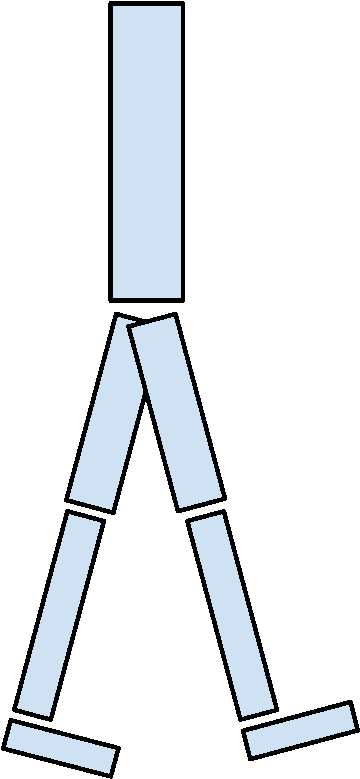
\includegraphics[width=0.2\linewidth]{../images/2D-Biped-crop.pdf} \\
	\caption{\label{figure:2d-biped} 2D planar biped. Each link has $3$ degrees of freedom $\langle x, y, \theta \rangle$.}
\end{figure}

\subsection{Character Construction}

I constructed a $7$ link biped with $21$ degrees of freedom~\ref{figure:2d-biped}. 
The root link is the waist of the character.
In \bulletPhysics, links are specified in world coordinates.
After the links are created, the constraints between the links are also defined in world coordinates.
 
Using the \Featherstone algorithm the links between rigid bodies are constructed in a hierarchical fashion. 
To create a new link, a new rigid body is created and then added to the system by specifying the id of the parent rigidbody and the child rigidbody. 
For example, if the torso is link $0$, then the left and right thigh links would specify their parent link as $0$.
Links are chained together with \emph{joints} in a method similar to links.
For each joint, the parent link needs to be set as well as the child link.
For a hinge joint, the axis of rotation also needs to be defined.
Last, the location of the joint, in world coordinates, is defined.
The system also has support for other types of joints, but they are not used in this project.

To drive the character, each joint has a function to set the current torque for a particular link. 
This torque is automatically applied to both links without the need to enforce the rotation separately.
The link torques will be controlled using Proportional Derivative (PD) controllers.
Each link is driven to a target angle using the formula $\tau = \Kp(\theta_{d}- \theta) - \Kd\dot{\theta} $.
Each non-symmetric joint has different values for \Kp and \Kd.

\begin{comment}
\begin{enumerate}
	\item Constructing a character
	\item Featherstone arrangement
	\item Controlling joints
	\item PD control on these joints
	\item getting a statue
	\item Using different solvers	
\end{enumerate}
\end{comment}

% Onto getting the character to walk

\subsection{Controller States}

The character controller uses a state machine to choose the particular angles toward which the biped should be driving. 
There are 4 states and these states are symmetric with respect to the left and right legs of the character.

\begin{comment}
\begin{table}
\centering
	\begin{tabular}{ c | c | c | c | c }
		            & state-0 & state-1 & state-2 & state-3 \\ \hline
         torso      &    0    &    0    &    0    & 0       \\
		 left-hip   &    0    &    0    &    0    & 0       \\
		 left-knee  &    0    &    0    &    0    & 0       \\
		left-ankle  &    0    &    0    &    0    & 0       \\
		 right-hip  &    0    &    0    &    0    & 0       \\
		right-knee  &    0    &    0    &    0    & 0       \\
		right-ankle &    0    &    0    &    0    & 0
	\end{tabular}
	\caption{\label{table:controler-values}}
\end{table}
\end{comment}

%The joint angles for each of the state are listed in Table~\ref{table:controler-values}.
The controller transitions between states for reasons: either a specific $\delta t$ has passed since the last transition, or there is a new foot contact.

% \todo{description of the states, maybe as picutres}

\subsection{Leg and Torso Control}

To give the biped better walking motion the legs and torso should have additional control and constraints.
The first of these is a desired angle for the torso of the biped in world coordinates.
The second is the swing leg of the controller is also driven toward a defined angle in world coordinates.
Last is a constraint that the torques for the torso (\torqueTorso) and swing leg (\torqueSwing) are equal to the torque generated by the stance leg (\torqueStance). 
This adds the constraint $\torqueStance = -\torqueTorso - \torqueSwing$.

\subsection{Feedback Control}

For additional balance control, linear feedback is used on the swing leg. This is done in the form:

\begin{equation}
\label{equation:feedback-law}
	\feedback = \defaultFeedbackTheta + \distanceFeedbackParam \distance + \velocityFeedbackParam \velocity
\end{equation}

with distance (\distance) and velocity (\velocity) feedback.
The distance \distance is calculated as the distance from the stance foot to the Centre of Motion (\COM), $\distance = -(\location{foot_{stance}} - \location{\COM})$.
The velocity \velocity is simply the velocity of the \COM.

\begin{comment}
\begin{enumerate}
	\item Some math for SIMBICON..
	\item implementing them in BulletPhysics
\end{enumerate}
\end{comment}

% 

\section{Results}
\label{sec:results}


	\noindent \textbf{Issues with PD controllers:}
	
	Finding the right settings for the PD controllers has been a difficult task. 
	This can be linked to difficulties of using the \Featherstone algorithm. 
	Typically, the torques on links are applied individually. 
	This is not true in this version of the \Featherstone algorithm. 
	No link operates independently and any torque applied to a motor at a joint is applied to both links attached at the joint. 
	This issue tends to propagate through the hierarchical chain of links. 
	
	\noindent \textbf{Use Dampening?}
	
	I did try to reduce some issues by applying additional linear and angular dampening. 
	Adding dampening only decreased the effect of the issues; they are still present.
	
	\noindent \textbf{Joint angle specification:}
	
	I found it was also difficult to work with joint angle specification in \bulletPhysics. Joint angles are constrained to be $0 \geq \theta \geq 2*\pi $. When a joint angle would wrap around, the PD controller would switch its driving direction. This typically results in the character gaining a significant amount of energy.
	
	\noindent \textbf{Detecting foot to ground contact:}
	
	Currently there are some issues with accurately detecting foot to ground contact. Ground contact is detected earlier than it should be. Investigation into the \bulletPhysics should lead to a solution to this issue.
	
	\noindent \textbf{Issues with defining the torso torque:}
	
	Again, because torques are automatically applied to both links, applying \torqueTorso is problematic. The method used in this work was to not specifically apply the torque to the torso but to instead only include it in stance leg torque computation.
	
	\noindent \textbf{Some simple walking motion:}
	
	Figure~\ref{figure:algorithm-steps} shows a sequence of the animation in $6$ clips. I think the character would be accepted into the Ministry of Silly Walks.
	
	\begin{figure}[!htb]
	\centering
	%trim=l b r t
	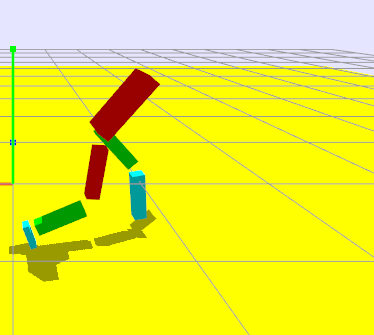
\includegraphics[width=0.45\linewidth]{../images/stepping/step-0.png} 
	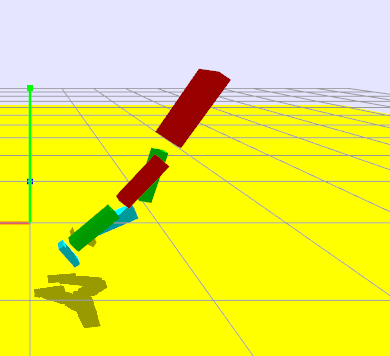
\includegraphics[width=0.45\linewidth]{../images/stepping/step-1.png} \\ 
	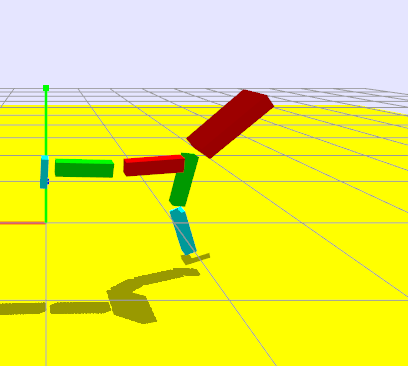
\includegraphics[width=0.45\linewidth]{../images/stepping/step-2.png}  
	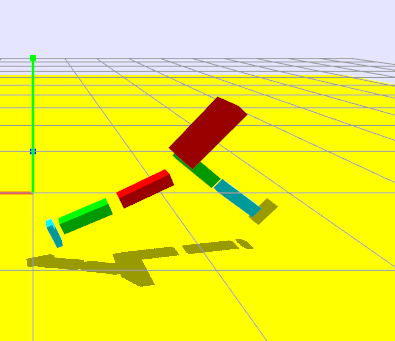
\includegraphics[width=0.45\linewidth]{../images/stepping/step-3.png}  \\
	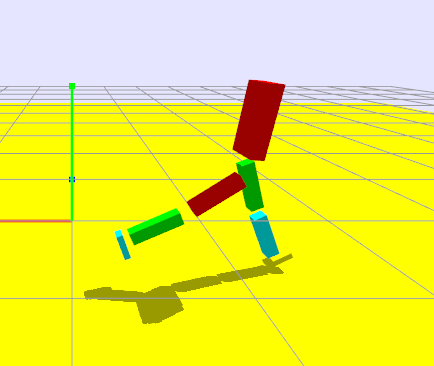
\includegraphics[width=0.45\linewidth]{../images/stepping/step-4.png}  
	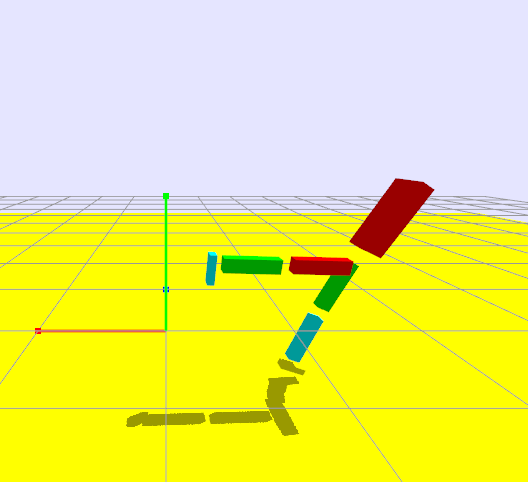
\includegraphics[width=0.45\linewidth]{../images/stepping/step-5.png}

	% \includegraphics[width=0.45\linewidth]{../images/steps/initial-mesh.pdf}  
	% (e) & (f) & (g) & (h)\\
	\caption{\label{figure:algorithm-steps} Sequence of captures of attempted walking behaviour. Order starts in the top left and proceeds to the right and then down.}
	\end{figure}
	
	\begin{figure}
		
	\end{figure}


% 
\section{Discussion}
\label{sec:Conclusion}

	\noindent \textbf{Was \bulletPhysics a good choice?}
	
	\bulletPhysics has been a great framework to use for this work. There are some design decisions I did not expect. However, I think the numerical stability and use of the \Featherstone algorithm are important advantages.

	\noindent \textbf{Different joint angle specification to help solve issues}
	
	I have found another method in \bulletPhysics to calculate relative joint angles that will hopefully help me eliminate some of the joint angle wrap around issues I have been having.
	

\bibliographystyle{named}
\bibliography{project}


%\addcontentsline{toc}{chapter}{Appendix}
% \input{report_appendix}

\end{document}